\documentclass[conference]{IEEEtran}
\IEEEoverridecommandlockouts

\usepackage{cite}
\usepackage{amsmath,amssymb,amsfonts}
\usepackage{algorithmic}
\usepackage{algorithm}
\usepackage{graphicx}
\usepackage{textcomp}
\usepackage{xcolor}
\usepackage{booktabs}
\usepackage{url}

\graphicspath{{figures/}}

\begin{document}

\title{Less Urgent, More Schedulable:\\ Local Deadline Assignment in Distributed EDF Systems}

\author{\IEEEauthorblockN{Juan M. Rivas and J. Javier Guti\'errez}
\IEEEauthorblockA{Universidad de Cantabria\\
Avda. de los Castros 48, 39005 Santander, Spain\\
Email: \{rivasjm, gutierrezjj\}@unican.es}}

\maketitle

\begin{abstract}
In distributed real-time systems, an end-to-end flow is a chain of tasks on
processors and messages on networks, and each resource orders its steps with a
local policy. \emph{We focus on resources scheduled by EDF.} Because the
end-to-end deadline of a flow is the only timing requirement, the local deadline
of each step is a free parameter that merely orders the step and fixes its
interference points.
Under holistic local-EDF response-time analysis, prior work reported a counterintuitive effect: assigning \emph{larger} local deadlines,
while keeping the end-to-end deadline fixed, increases the number of systems the
analysis certifies as schedulable. The trend is not monotone, since the optimum
is interior. We observe the effect through this analysis rather than claim it for EDF in
general, and we study it systematically. An interfering task's local deadline
caps its demand in the interference bound, so a later deadline makes the task
interfere in fewer deadline windows. We exploit
this with WAD, a one-pass closed-form rule, and with WAD-Adapt, which adds three
correction passes. To measure how much these cheap rules leave on the table, we
also present RTA-CD, a coordinate-descent search guided by the analysis, as a
per-instance ceiling. In a synthetic evaluation with 1000 systems per size,
WAD-Adapt reaches 928 and 798 schedulable systems, against 964 and 883 for
RTA-CD. That is 96.3\% and 90.4\% of the ceiling, with 47.5 and 27.9 times
lower runtime. Since the analysis is a sufficient (pessimistic) test, a system it
certifies is genuinely schedulable, although a tighter analysis could change the
size of the gain and the position of the optimum.
\end{abstract}

\begin{IEEEkeywords}
Distributed real-time systems, EDF scheduling, deadline assignment,
response-time analysis, scheduling parameter optimization.
\end{IEEEkeywords}

\section{Introduction}
\label{sec:intro}

In distributed real-time systems, an application is often modeled as a set of
\emph{flows} with end-to-end deadlines. A flow is a chain of steps, where each
step is either a task computed on a processor or a message transmitted on a
network. The steps of a flow may run on different processors and networks, and
each resource applies a local scheduling policy.

Under \emph{local EDF} (LC-EDF), each resource schedules with its own clock, so
no synchronized global time base is assumed. Each step has a \emph{local
deadline} that defines both its EDF order on the resource and the deadline points
at which its interference is accounted for. Schedulability is defined by the
flow's \emph{end-to-end} deadline, and a step's local deadline need not
correspond to any real requirement. It is therefore a \emph{free parameter}, and
the quality of a deadline-assignment heuristic largely determines how many
systems can be scheduled.

Classical heuristics assign local deadlines proportional to worst-case execution
times (\emph{proportional deadlines}, PD)~\cite{dinatale}. Others refine them
iteratively, such as the HOSPA heuristic~\cite{hospa}, the EDF adaptation of the
fixed-priority HOPA heuristic~\cite{hopa}. These heuristics treat the local
deadlines as \emph{budgets}, making each task as urgent as the flow's end-to-end
deadline allows. We start from the opposite observation, first reported
in~\cite{rivas15}.

\smallskip
\noindent\textbf{Observation} (first reported in~\cite{rivas15}, which
summarized it as ``more haste, less speed''). \emph{Under holistic local-EDF
response-time analysis, increasing local scheduling deadlines while keeping the
flow's end-to-end deadline fixed raises the number of systems the analysis
certifies, up to an interior optimum beyond which it falls again.}
That work proposed two basic techniques: LC-EDF-DS scales the end-to-end
deadline, and LC-EDF-GSD uses the global cumulative deadlines. We generalize
both with a finer two-parameter grid, which lets us study the phenomenon in more
detail.

This is surprising, because enlarging a local deadline looks like it should
\emph{hurt} its task, yet it helps the system. We do not claim the phenomenon.
Our contributions beyond~\cite{rivas15} are the demand-cap mechanism, the
back-loaded shape with the closed-form rules WAD and WAD-Adapt, the search
ceiling RTA-CD, and a systematic study.

\smallskip\noindent\textbf{Problem.} We seek a deadline-assignment rule that is
\emph{cheap} and \emph{explainable}, and that maximizes the number of schedulable
systems in a fixed benchmark. Cheap means a closed form or a fixed number of
analysis passes, with no per-instance search, whereas explainable means that its
structure follows from the analysis. We also ask how much of a per-instance
search's count such a rule captures, and at what cost.

\smallskip\noindent\textbf{Contributions.}
\begin{itemize}
\item \textbf{C1.} Taking the effect of~\cite{rivas15} as given, we identify the
channel through which larger local deadlines help. An interfering task's local
deadline acts as a \emph{demand cap} in the interference bound, so a later local
deadline makes it interfere in fewer deadline windows. We prove that the
interference term is non-increasing in the interferer's local deadline (Prop.~1),
and we measure its net effect on schedulability
(Sections~\ref{sec:obs}--\ref{sec:why}).
\item \textbf{C2.} We propose \emph{WAD}, a one-pass closed-form rule, and
\emph{WAD-Adapt}, which adds a fixed number of correction passes
(Sections~\ref{sec:rule}--\ref{sec:eval}).
\item \textbf{C3.} We present \emph{RTA-CD}, a coordinate search guided by the
analysis and used as a per-instance ceiling, and we measure how much of that
ceiling the cheap rules capture and at what cost (Section~\ref{sec:eval}).
\item \textbf{C4.} We ablate the effect by comparing order against magnitude,
budget against overspend, and the shape of the deadlines at equal spend. The
effect holds across system shapes and generator seeds. We also give a variant
that respects $\sum_i d_i\le D_f$ (Section~\ref{sec:ablation}).
\item \textbf{C5.} We state the limitations: the rules exploit an
\emph{approximate} bound, and RTA-CD can assign deadlines below the execution
time (Section~\ref{sec:discussion}).
\end{itemize}

\noindent The rest of the paper recalls the model and analysis, states and
explains the observation, derives the rules, and evaluates them.

\section{Related Work}
\label{sec:related}

\smallskip\noindent\textbf{Deadline assignment.} Assigning local deadlines under
EDF ranges from proportional and end-to-end deadline
propagation~\cite{dinatale} to iterative heuristics such as HOSPA~\cite{hospa},
the EDF adaptation of the fixed-priority HOPA heuristic~\cite{hopa}. These
methods treat the local deadlines as budgets to be spent within the flow's
end-to-end deadline. We show instead that a local deadline is better used as a
\emph{demand cap} in the interference bound, which a generous, back-loaded
assignment exploits, and we provide a closed-form rule for it.

\smallskip\noindent\textbf{Overspending the end-to-end deadline.} The closest
prior work is~\cite{rivas15}, by the same authors. It showed that under LC-EDF,
assigning \emph{larger} scheduling deadlines yields lower worst-case response
times and better schedulability (``more haste, less speed''), and it proposed two
overspending techniques. LC-EDF-DS scales the end-to-end deadline by a factor
(our uniform scale $\lambda$), whereas LC-EDF-GSD uses the global cumulative
scheduling deadlines (our $\gamma{=}1$). The phenomenon and these two basic families are
therefore not new here, and our contributions beyond~\cite{rivas15} are
threefold. (i) The demand-cap mechanism in the interference bound, proved
(Prop.~1) and tested by a counterfactual. (ii) The partial-globalization,
back-loaded shape and the resulting closed-form rule WAD, its correction variant
WAD-Adapt, and the RTA-CD search ceiling. (iii) A systematic study covering the
interior optimum, order versus magnitude, the shape of the deadlines, a
budget-feasible variant, and generalization.

\smallskip\noindent\textbf{The analysis.} We build on the holistic analysis for
distributed, EDF-scheduled systems~\cite{audsley,holistic,palencia}, which
accounts for release jitter. We also use arbitrary-deadline EDF
results~\cite{spuri,lehozcky}, and partitioned (per-processor) EDF is surveyed
in~\cite{davis}. Our contribution is a structural reading of this analysis and
not a new analysis.

\section{System Model and Holistic Local-EDF Analysis}
\label{sec:model}

\subsection{Model}
A system is a set of \emph{processing resources} and a set $\mathcal{F}$ of
\emph{end-to-end flows}. The resources are one or more processors and one or more
communication \emph{networks}. A flow $f\!\in\!\mathcal{F}$ is an ordered chain of
$n_f$ steps, indexed $k=0,\dots,n_f{-}1$. We write $j\prec k$ when $j$ precedes
$k$ in the flow. A flow has a period $T_f$ and an end-to-end deadline $D_f$, and
each of its steps is either a \emph{task}, executed on a processor, or a
\emph{message}, transmitted on a network. Steps are statically mapped onto
resources.

In the systems we study, every resource schedules its steps by \emph{local
EDF}~\cite{liu}, that is, by ascending local \emph{absolute} deadlines. The
network is scheduled as a resource in exactly the same way. We therefore use
``task'' and ``processor'' for a step and its resource of either kind, so that a
message on a network is handled as a task on a processor.

Throughout, $a$ denotes the analyzed task and $i$ ranges over the other tasks of
its resource. The indices $k$ and $j$ denote positions within a flow. A task has
worst-case execution (or transmission) time $C$ and a \emph{local deadline} $d$,
which is the local \emph{scheduling} deadline the EDF dispatcher uses and the
parameter we assign. We write $C_a,d_a$ or $C_k,d_k$ depending on how the
task is indexed. Its \emph{release jitter} $J_a$ is the maximum response time of
its predecessors in the flow ($J_a=0$ for the first task). The end-to-end
response time of a flow is the response time $R_{\mathrm{last}(f)}$ of its last
step, and the flow is \emph{schedulable} iff $R_{\mathrm{last}(f)}\le D_f$. The
deadline $d_a$ encodes the EDF order but is not itself a schedulability
requirement.

\subsection{Response-time analysis}
We use the holistic local-EDF analysis of~\cite{hospa} (equations numbered as in
that reference). For a task $a$ on a processor, the \emph{busy period} is the
fixed point (eq.~(5))
\begin{equation}
L_a = \Big\lceil \tfrac{L_a}{T_a}\Big\rceil C_a
      + \sum_{i\ne a} \Big\lceil \tfrac{L_a+J_i}{T_i}\Big\rceil C_i ,
\end{equation}
where the sum runs over the other tasks $i$ of the processor. The interference a
task $i$ contributes to a window ending at deadline point $\psi$ is (eq.~(1))
\begin{equation}
w_i(t,\psi) =
\begin{cases}
\min\!\Big(\big\lceil \tfrac{t+J_i}{T_i}\big\rceil,\;
          \big\lfloor \tfrac{J_i + \psi - d_i}{T_i}\big\rfloor+1\Big) C_i, & \psi \ge d_i,\\[2pt]
0, & \psi < d_i .
\end{cases}
\label{eq:wi}
\end{equation}
The analysis then iterates over the \emph{deadline points} $\psi$ of the
processor (eqs.~(4),(6)) and the activation indices $p=1,2,\dots$. For each pair
it solves the fixed point (eq.~(8))
\begin{equation}
w_{a,p}= p\,C_a + \sum_{i\ne a} w_i\!\left(w_{a,p},\psi\right),
\end{equation}
and takes
\begin{equation}
r_{a,p}= w_{a,p} - \psi + d_a + J_a,\qquad
R_a = \max_{p,\psi} r_{a,p}. \label{eq:ra}
\end{equation}
Since $J_a$ is the response time of $a$'s predecessors, the whole computation
is a fixed point across the flow, which we evaluate exactly as in~\cite{hospa}.

\smallskip\noindent\textbf{Scope and assumptions.} As in~\cite{hospa}, flows are
periodic chains with a fixed task-to-processor mapping and no offsets or phases.
A task's release jitter is exactly the maximum response time of its
predecessors. Schedulability here means ``certified by the analysis above'', and
that analysis is a \emph{sufficient} (pessimistic) test. When it certifies a
system, every flow meets its end-to-end deadline, but it may fail to certify some
systems that are in fact schedulable. The local deadlines are unconstrained free
parameters, so nothing forces $\sum_i d_i\le D_f$, and our rules sometimes
exploit that (Section~\ref{sec:discussion}).

\section{The Observation: Larger Local Deadlines Help}
\label{sec:obs}

This section reproduces, on our benchmark, the effect first reported
in~\cite{rivas15}, namely that larger local deadlines raise the number of
schedulable systems. We assign local deadlines with two one-parameter families
whose endpoints are the techniques of~\cite{rivas15} (uniform scale: LC-EDF-DS,
$\gamma{=}1$: LC-EDF-GSD). Both are built on the proportional share
$s_k = C_k\,D_f/\sum_{j\in f}C_j$ of task $k$ in its flow $f$:
\begin{itemize}
\item \emph{partial globalization} $\gamma$:
$d_k = s_k + \gamma \sum_{j \prec k} s_j$. Here $\gamma{=}0$ is PD, and
$\gamma{=}1$ makes the deadlines cumulative along the chain.
\item \emph{uniform scale} $\lambda$: $d_k = \lambda\, s_k$.
\end{itemize}
Fig.~\ref{fig:obs} reports the number of schedulable instances out of 1000 on
the benchmark of Section~\ref{sec:eval}. The proportional baseline PD gives 706,
while both families peak in the interior ($\gamma^\star\!\approx\!0.3$--$0.5$:
814--815, $\lambda^\star\!\approx\!2$: 808) and degrade afterwards
($\gamma{=}1$: 745, $\lambda{=}5$: 774). Asking tasks to run later therefore
helps, but only up to a point.

\begin{figure}[t]
\centering
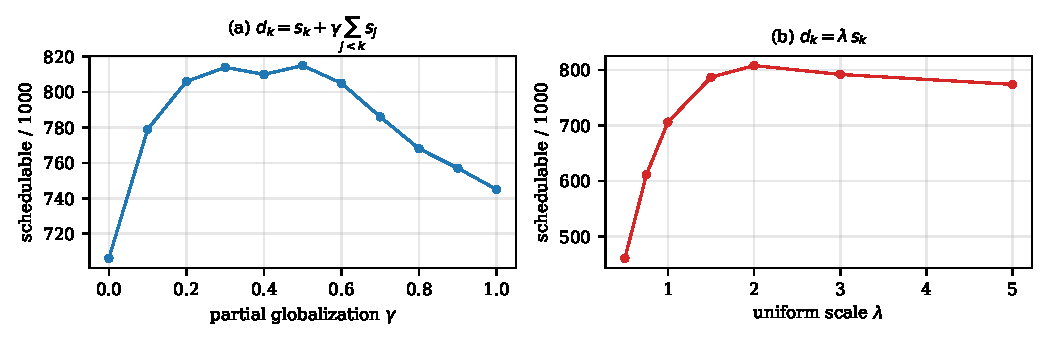
\includegraphics[width=\columnwidth]{fig1_observation.pdf}
\caption{Schedulable systems (out of 1000, size-15 benchmark) against (a) the
partial-globalization coefficient $\gamma$ and (b) the uniform deadline scale
$\lambda$. Both curves peak at an interior value. The points $\gamma=0$ and
$\lambda=1$ correspond to PD.}
\label{fig:obs}
\end{figure}

\section{Why: The Demand Cap in the Interference Bound}
\label{sec:why}

The effect of Section~\ref{sec:obs} was reported in~\cite{rivas15}. This section
explains it through the analysis. The only place where an \emph{interfering}
task's local deadline $d_i$ appears in the analysis is the second argument of the
minimum in \eqref{eq:wi}. Write
\begin{equation}
\delta_i(\psi) =
\begin{cases}
\big\lfloor (J_i + \psi - d_i)/T_i \big\rfloor + 1, & \psi \ge d_i,\\
0, & \psi < d_i.
\end{cases}
\label{eq:cap}
\end{equation}
Then $w_i(t,\psi)=\min(\lceil (t+J_i)/T_i\rceil,\ \delta_i(\psi))\,C_i$.

\begin{quote}
\textbf{Proposition 1.} \emph{For fixed $t$ and $\psi$, $w_i(t,\psi)$ is
non-increasing in $d_i$, and $w_i(t,\psi)=0$ whenever $d_i>\psi$.}
\end{quote}
\noindent\emph{Proof.} $\delta_i(\psi)$ is a non-increasing, integer-valued step
function of $d_i$ (a floor of a decreasing affine function). It equals $0$ for
$d_i>\psi$. The minimum with the non-negative, $d_i$-independent activation bound
preserves monotonicity. $\square$

Hence a later local deadline reduces the interference the bound attributes to a
task, even though $d_i$ belongs to an \emph{interferer} and not to the analyzed
task, and once $d_i>\psi$ the task is ignored entirely in that window.

\smallskip\noindent\textbf{Example.} Two single-task flows, $C_a=2$, $C_b=3$,
$T=10$, on one processor, with $d_a<d_b$. The analysis gives
$R_a=\max(C_a,\,C_a+C_b-(d_b-d_a))$ and $R_b=C_a+C_b=5$
(Appendix~\ref{app:deriv}). Enlarging $b$'s local deadline reduces $a$'s
response one-for-one until $d_b-d_a\ge C_b$, after which $R_a=C_a$. A later
deadline on an \emph{interferer} thus strictly helps its processor-mates.

The analyzed task's own deadline $d_a$ enters differently. In \eqref{eq:ra}, at
the worst deadline point $\psi=(p{-}1)T_a+d_a$ the additive $+d_a$ cancels
exactly: $r_{a,p}=w_{a,p}-(p{-}1)T_a+J_a$. The residual dependence is through
$w_{a,p}$, that is, through which interferers fall inside the window and through
$\delta_i$, so $d_a$ is not ``time the task is allowed'' but rather selects the
window in which the task is analyzed.

Two opposing effects produce the non-monotone behavior of Fig.~\ref{fig:obs}.
A larger interferer deadline $d_i$ reduces interference, whereas a larger analyzed
deadline $d_a$ shifts the analysis window and changes the flow's budget
allocation. The benefit does \emph{not} require enlarging every deadline
uniformly, because which task is made late matters as much as by how much
(Section~\ref{sec:ablation}).

Prop.~1 is a statement about the pointwise interference term at fixed $(t,\psi)$.
In the full analysis, the deadline points $\psi$ are themselves generated from
the local deadlines, and raising $d_i$ also raises the jitter of its successors,
so the net effect is empirical. Prop.~1 identifies the \emph{channel} of the
effect and not the location of the optimum. A counterfactual that removes only
the cap's floor term shows no interior optimum, and removing the cap entirely
degenerates the analysis (Table~\ref{tab:cf}).

\begin{table}[t]
\centering
\caption{Counterfactual analyses (schedulable / 1000, size-15 benchmark): the
uniform-scale family $d_k=\lambda s_k$ for several $\lambda$, and one-pass WAD.
Removing the cap removes the effect.}
\label{tab:cf}
\begin{tabular}{lrrr}
\toprule
 & full & cutoff only & no cap \\
\midrule
$\lambda=0.5$ & 460 & 195 & 0 \\
$\lambda=1$   & 706 & 386 & 0 \\
$\lambda=2$   & 808 & 572 & 0 \\
$\lambda=3$   & 794 & 652 & 0 \\
$\lambda=5$   & 775 & 701 & 0 \\
WAD           & 875 & 644 & 0 \\
\bottomrule
\end{tabular}
\end{table}

The demand cap is a property of the bound \eqref{eq:wi}. Since the analysis is a
\emph{sufficient} (pessimistic) test, a system it certifies is genuinely
schedulable, and the gain we report is therefore an increase in \emph{guaranteed}
schedulability. The cap belongs to this test's precision, since a lower-priority
task still executes and could still interfere in a busy window. The size of the
gain and the location of the interior optimum may differ under a tighter
analysis, as Section~\ref{sec:discussion} discusses.

\section{Exploiting the Observation: A Cheap Assignment Rule}
\label{sec:rule}

The observation suggests two ingredients. First, interference is capped by the
\emph{interferer's} deadline. Later tasks have their ``true'' completion point at
the end of the chain, so they should get later local deadlines, which
\emph{back-loads} the flow budget and reduces the interference imposed by
downstream tasks. Second, a task's response exceeds its own execution because it
also carries interference, so each share must be scaled up by a safety factor.
Together these yield the one-pass rule \textbf{WAD} (work-and-position aware):
\begin{equation}
d_k = D_f\Big( \kappa_{\mathrm{w}}\,\frac{C_k}{\sum_{j\in f} C_j}
      + \kappa_{\mathrm{p}}\,\frac{k}{n_f-1} \Big),\quad k=0,\dots,n_f{-}1,
\label{eq:wad}
\end{equation}
with constants $\kappa_{\mathrm{w}}=1.6$ and $\kappa_{\mathrm{p}}=0.4$ chosen by a
grid search (Fig.~\ref{fig:sens}).

The first term is proportional (work), while the second is a position ramp that
shifts budget toward the later tasks. With $n_f=1$ the ramp term is set to $1$, so
a single-task flow receives
$d=(\kappa_{\mathrm{w}}{+}\kappa_{\mathrm{p}})D_f=2D_f$, which is harmless
because it has no successors to delay. WAD is a single pass over the flows, with
no analysis and no search, and on the benchmark it scores 875.

\textbf{WAD-Adapt} adds a fixed number $N_{\mathrm{pass}}=3$ of correction passes.
Each pass (1) analyzes the system with a very large response-time limit, so that
every flow's untruncated response $R_f$ is available, and (2) rescales \emph{all}
the local deadlines of each flow by
\begin{equation}
\phi_f = \min\!\Big(\max\!\big((D_f/R_f)^{\alpha},\,\phi_{\min}\big),\,
\phi_{\max}\Big),
\label{eq:adapt}
\end{equation}
with $\alpha=0.5$, $\phi_{\min}=0.75$ and $\phi_{\max}=1.25$. A flow that
overshoots shrinks, whereas a flow with slack grows, which by Prop.~1 further
suppresses the interference it imposes on its processor-mates. The exponent damps
the step, and the clamp acts as a trust region.

WAD-Adapt scores 928. Because it performs a fixed number of passes, it is not a
search, but it is no longer a closed form, and neither rule uses randomness. The
constants ($\alpha=0.5$, $\phi_{\min/\max}=0.75/1.25$, $N_{\mathrm{pass}}=3$) were
chosen on the size-15 benchmark, and the score varies by only a few systems for
$N_{\mathrm{pass}}\in\{2,3,4\}$.

\textbf{WAD-Budget} is the budget-feasible variant of WAD-Adapt, in which every
flow's local deadlines are projected onto $\sum_k d_k=D_f$ after each pass. WAD,
WAD-Adapt and WAD-Budget form the \emph{WAD family}.

\smallskip\noindent\textbf{Cost.} WAD runs in one pass over the flows ($O(n_f)$ per
flow, no analysis). WAD-Adapt runs $N_{\mathrm{pass}}{=}3$ analyses of the whole
system, so the analysis dominates its cost. Unlike a search, it makes a fixed
number of passes that does not grow with the difficulty of the instance.

\section{Evaluation}
\label{sec:eval}

\subsection{Protocol}
Each system has $15$ or $25$ tasks ($5$ flows of $3$ or $5$ tasks) mapped onto
$3$ or $5$ processors. We call the two scenarios EDF-15 and EDF-25. Periods are
drawn log-uniformly in $[100,1000]$. Each flow's end-to-end deadline is uniform
in $[0.5\,n_f T_f,\,n_f T_f]$. Per-task utilizations are drawn with
UUNIFAST~\cite{uunifast} to reach a target load, and tasks are assigned
round-robin, in decreasing order of utilization, so that every processor gets the
same number of tasks.

Each scenario has $50$ systems (generator seed 42) swept over $20$ utilization
levels in $[0.5,0.9]$, which gives $1000$ instances per size. The metric is the
number of schedulable instances. We report the rules of Section~\ref{sec:rule}
(WAD, WAD-Adapt, WAD-Budget) against the reference methods below, and we ran all
methods ourselves, on the same machine.

\subsection{Reference methods}
We report PD (baseline), the classical EQF and EQS assignments~\cite{dinatale},
HOSPA, and RTA-CD.

RTA-CD (CD for coordinate descent) is a per-instance search that we use as a
strong reference. It starts from an analytic assignment that favors flows whose
deadline is tight relative to their period and then performs multiplicative
coordinate descent on the local deadlines. The objective is
$\sum_f \max(0, R_f/D_f-1)$, computed by the analysis itself with a relaxed
response-time limit, and the search stops as soon as the exact analysis (limit
factor $1$) reports the system schedulable.

RTA-CD is deterministic. It runs at most $16$ sweeps of the coordinate descent
and stops earlier if a sweep improves nothing, while a safety guard of $1200$\,s
limits a single pathological sweep, a guard that is not reached on any instance.
The analytic start alone schedules $782$ of $1000$ instances on size~15 and $654$
on size~25. One instance per size reaches the $16$-sweep limit and is not schedulable.
The search never ends worse than its starting point.

\begin{algorithm}[t]
\caption{RTA-CD (one instance)}
\label{alg:rta}
\begin{algorithmic}[1]
\REQUIRE system; factors $\mathcal{M}=\{0.5,0.7,\dots,2.3\}$; $N_{\mathrm{sweep}}=16$
\ENSURE a local-deadline assignment $d$
\STATE $d \leftarrow$ analytic start (favoring flows with tight $D_f/P_f$)
\STATE $v \leftarrow \sum_f \max(0,\,R_f/D_f-1)$ with a relaxed limit factor
\IF{the exact analysis declares the system schedulable}
  \STATE \textbf{return} $d$
\ENDIF
\FOR{$s = 1$ \TO $N_{\mathrm{sweep}}$}
  \STATE improved $\leftarrow$ false
  \FOR{each task $i$}
    \FOR{each $m\in\mathcal{M}$}
      \IF{$m\cdot d_i$ lowers $v$}
        \STATE $d_i \leftarrow m\cdot d_i$
        \STATE improved $\leftarrow$ true
      \ENDIF
    \ENDFOR
  \ENDFOR
  \IF{not improved} \STATE \textbf{return} $d$ \ENDIF
  \IF{the exact analysis declares the system schedulable}
    \STATE \textbf{return} $d$
  \ENDIF
\ENDFOR
\STATE \textbf{return} the best $d$ found
\end{algorithmic}
\end{algorithm}

\subsection{Results}
Tables~\ref{tab:main} and~\ref{tab:25} and Figs.~\ref{fig:sched}--\ref{fig:time}
summarize the results, and Table~\ref{tab:dl} lists the deadlines the rules
assign. On size~15, WAD (one pass) reaches 875, WAD-Adapt 928 and RTA-CD 964,
while HOSPA reaches 840. On the harder size~25, WAD reaches 718, WAD-Adapt 798 and
RTA-CD 883, against 592 for HOSPA.

The classical EQF and EQS assignments are the strongest cheap baselines:
they score 783 and 734 on size~15 and 656 and 552 on size~25, all above PD. On
size~25, EQF (656) is above HOSPA (592) while EQS (552) is below it, but both
remain below WAD and WAD-Adapt. The budget-feasible WAD-Budget still beats PD (776
versus 706 on size~15, 478 versus 438 on size~25).

\smallskip\noindent\textbf{How much of the ceiling the cheap rule captures.}
RTA-CD is the strongest method we ran, so we use it as a ceiling. WAD-Adapt
reaches 928 of its 964 systems on size~15 (96.3\%) and 798 of its 883 on size~25
(90.4\%), while RTA-CD costs 47.5 and 27.9 times more per system than WAD-Adapt.
The two sets are not disjoint, since relative to WAD-Adapt, RTA-CD schedules 38
and 86 additional systems and fails on 2 and 1 that WAD-Adapt schedules. RTA-CD
also exceeds HOSPA by 124 and 291 systems. The ceiling is a search result and not
a proven optimum.

The efficiency plots (Fig.~\ref{fig:eff}) make the trade-off explicit. WAD and EQF
are Pareto-optimal among the fast methods, whereas RTA-CD trades time for the last
instances.

\begin{table}[t]
\centering
\caption{EDF-15 results (1000 systems): schedulable count and mean time per
system in seconds. All methods were run by us, on the same machine.}
\label{tab:main}
\begin{tabular}{lrr}
\toprule
method & schedulable & mean time (s) \\
\midrule
PD                 & 706 & 0.0116 \\
EQF                & 783 & 0.0050 \\
EQS                & 734 & 0.0056 \\
HOSPA              & 840 & 3.8487 \\
\midrule
WAD                & 875 & 0.0075 \\
WAD-Adapt          & 928 & 0.0496 \\
WAD-Budget         & 776 & 0.1494 \\
RTA-CD             & 964 & 2.3565 \\
\bottomrule
\end{tabular}
\end{table}

\begin{table}[t]
\centering
\caption{EDF-25 results (1000 systems): schedulable count and mean time per
system in seconds. All methods were run by us, on the same machine.}
\label{tab:25}
\begin{tabular}{lrr}
\toprule
method & schedulable & mean time (s) \\
\midrule
PD                 & 438 & 0.0181 \\
EQF                & 656 & 0.0124 \\
EQS                & 552 & 0.0116 \\
HOSPA              & 592 & 32.4682 \\
\midrule
WAD                & 718 & 0.0191 \\
WAD-Adapt          & 798 & 0.7332 \\
WAD-Budget         & 478 & 2.6427 \\
RTA-CD             & 883 & 20.4336 \\
\bottomrule
\end{tabular}
\end{table}

\begin{table}[t]
\centering
\caption{Deadline statistics of the WAD family. Minimum $d_i/C_i$ and
mean/maximum $\sum_i d_i/D_f$ per flow. EDF-15 is the full benchmark, and EDF-25
is sampled at 5 levels. WAD-Budget has $\sum_i d_i=D_f$ by construction.}
\label{tab:dl}
\begin{tabular}{lrrr}
\toprule
 & WAD & WAD-Adapt & WAD-Budget \\
\midrule
min $d_i/C_i$ (EDF-15)            & 2.12 & 1.08 & 0.96 \\
mean $\sum_i d_i/D_f$ (EDF-15)    & 2.2  & 3.95 & 1.0 \\
mean $\sum_i d_i/D_f$ (EDF-25)    & 2.6  & 4.49 & 1.0 \\
max $\sum_i d_i/D_f$ (EDF-25)     & 2.6  & 5.08 & 1.0 \\
\bottomrule
\end{tabular}
\end{table}

\begin{figure}[t]
\centering
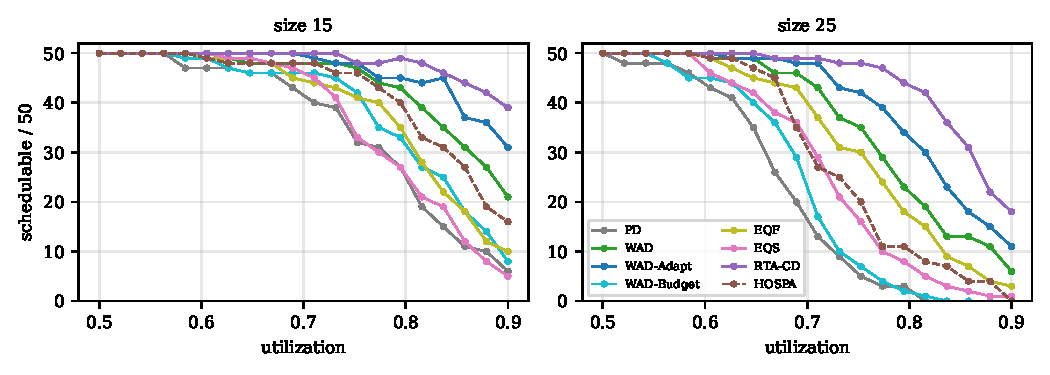
\includegraphics[width=\columnwidth]{fig2_schedulables.pdf}
\caption{Schedulable systems per utilization level for EDF-15 (left) and EDF-25
(right). There are 50 systems per level.}
\label{fig:sched}
\end{figure}

\begin{figure}[t]
\centering
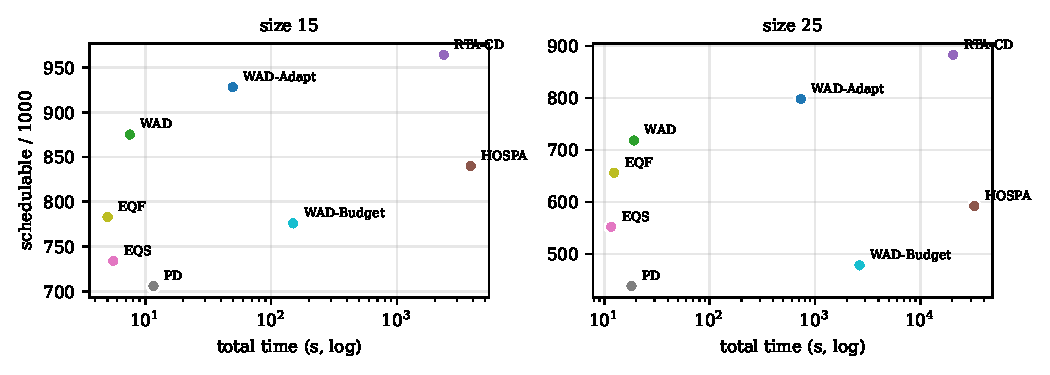
\includegraphics[width=\columnwidth]{fig3_efficiency.pdf}
\caption{Efficiency: total schedulable systems against total execution time (log
scale), EDF-15 (left) and EDF-25 (right). Points toward the upper left are
better.}
\label{fig:eff}
\end{figure}

\begin{figure}[t]
\centering
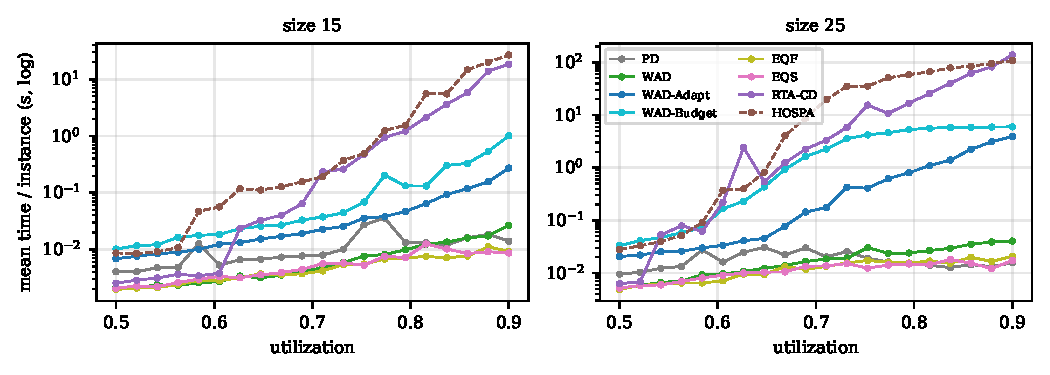
\includegraphics[width=\columnwidth]{fig4_times.pdf}
\caption{Mean execution time per system against utilization (log scale), EDF-15
and EDF-25.}
\label{fig:time}
\end{figure}

\subsection{Robustness to the seed and the constants}
The benchmark is generated from a fixed seed, so the rule and its constants might
overfit that seed. Table~\ref{tab:seed} varies the generator seed, and WAD stays
within $853$--$875$ while WAD-Adapt stays within $913$--$928$. The result
therefore does not depend on the particular seed.

The constants $\kappa_{\mathrm{w}}$ and $\kappa_{\mathrm{p}}$ were chosen on the
seed-42 benchmark (Fig.~\ref{fig:sens}). The figure shows a broad plateau, maximal
at $(\kappa_{\mathrm{w}},\kappa_{\mathrm{p}})=(1.6,0.4)$, which is the WAD
setting and scores 875.

\begin{table}[t]
\centering
\caption{Seed robustness (schedulable / 1000).}
\label{tab:seed}
\begin{tabular}{lcccc}
\toprule
rule & seed 1 & seed 7 & seed 42 & seed 123 \\
\midrule
PD         & 710 & 767 & 706 & 726 \\
WAD        & 863 & 853 & 875 & 867 \\
WAD-Adapt  & 926 & 913 & 928 & 921 \\
WAD-Budget & 764 & 767 & 776 & 760 \\
\bottomrule
\end{tabular}
\end{table}

\begin{figure}[t]
\centering
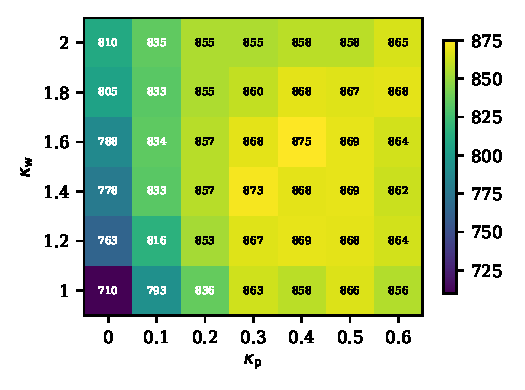
\includegraphics[width=0.78\columnwidth]{fig5_sensitivity.pdf}
\caption{Schedulable systems for one-pass WAD on EDF-15 (seed 42) over a grid of
the constants $\kappa_{\mathrm{w}}$ and $\kappa_{\mathrm{p}}$.}
\label{fig:sens}
\end{figure}

\section{Ablation and Generalization}
\label{sec:ablation}

\subsection{Order versus magnitude}
Is the gain from \emph{ordering} the deadlines differently, or from their
\emph{magnitude}? In the experiments of Fig.~\ref{fig:obs}, the original ordering
is best, and every other permutation of the proportional shares performs much
worse. Shuffling the tuned WAD deadlines within each flow improved only $19$ of
the $1000$ instances (over $20$ random shuffles each) and worsened $11{,}204$ of
the $20{,}000$ shuffles. Order therefore matters enormously, though it is not
literally never helpful.

The back-loaded \emph{shape} alone and the \emph{magnitude} alone each help. The
2-D grid of $(\gamma,\lambda)$ peaks at $(\gamma,\lambda)=(0.2,2.0)$ with 862
schedulable systems, which is higher than either family alone, so both levers
contribute.

\subsection{Is it only budget overspending?}
Enlarging deadlines spends more than the flow's end-to-end deadline
($\sum_i d_i > D_f$). Is the whole effect an artifact of ``spending more''? The
budget-feasible WAD-Budget (Section~\ref{sec:rule}) still reaches 776 on size~15
and 478 on size~25, which is well above PD (706/438) though below the
unconstrained WAD-Adapt (928/798). For this rule, overspending is worth on the
order of $150$ instances at size~15 ($\sim$16\%). The direction is genuine, but
part of the score is bought by the freedom to overspend, and closing the gap to
the best budget-feasible assignment is open.

\subsection{Shape of the assigned deadlines}
Where do the assignments sit in the $(\gamma,\lambda)$ family of
Section~\ref{sec:obs}? Table~\ref{tab:shape} fits each flow's deadlines to
$d_k\approx\lambda s_k+\lambda\gamma\sum_{j\prec k}s_j$ and reports medians.

The WAD family fits with $\gamma=0.27$ on size~15 and $0.24$ on size~25, and
$R^2$ close to $0.99$. The correction raises $\lambda$ (from $1.67$ to $3.15$ on
size~15), whereas WAD-Budget scales down so that it spends exactly $D_f$.

RTA-CD has a median $\gamma$ of $0$, which comes from its analytic start, since
that start is proportional by construction ($d_i\propto C_i$, so $\gamma=0$ and
$R^2=1$) and already schedules $782$ and $654$ instances. On the instances that go
on to the descent, the median $\gamma$ is still low, $0.07$, with a median $R^2$ of
$0.96$ on size~15 and $0.85$ on size~25. The spread is large (the 90th percentile
of $\gamma$ is $1.09$ and $0.55$), but we see no systematic back-loading.

RTA-CD does not win by spending more, since its mean spend ($1.87$ and $2.71$) is
similar to that of WAD ($2.20$ and $2.60$). It wins by distributing the spend
across flows, and its per-flow $\lambda$ has an interquartile range of about
$0.49$ and $0.79$.

\begin{table}[t]
\centering
\caption{Where each assignment sits in the two-lever family of
Section~\ref{sec:obs}. Median over flows of the least-squares fit
$d_k\approx\lambda s_k+\lambda\gamma\sum_{j\prec k}s_j$, median $R^2$, mean
spend $\sum_i d_i/D_f$ and minimum $d_i/C_i$. Size~25 uses the same five
utilization levels as Table~\ref{tab:dl}. RTA-CD's median $\gamma=0$ is dominated
by the instances its analytic start already schedules, which are proportional by
construction. On the instances that need the descent, the median $\gamma$ is
$0.07$ with $R^2=0.96$ (size~15) and $0.85$ (size~25).}
\label{tab:shape}
\begin{tabular}{lrrrrr}
\toprule
 & $\gamma$ & $\lambda$ & $R^2$ & $\sum_i d_i/D_f$ & $\min d_i/C_i$ \\
\midrule
\multicolumn{6}{l}{\emph{EDF-15}}\\
WAD          & 0.27 & 1.67 & 0.995 & 2.20 & 2.12 \\
WAD-Adapt    & 0.27 & 3.15 & 0.995 & 3.95 & 1.08 \\
WAD-Budget   & 0.27 & 0.76 & 0.995 & 1.00 & 0.96 \\
RTA-CD       & 0.00 & 1.85 & 1.000 & 1.87 & 0.00 \\
\midrule
\multicolumn{6}{l}{\emph{EDF-25}}\\
WAD          & 0.24 & 1.75 & 0.988 & 2.60 & 3.01 \\
WAD-Adapt    & 0.24 & 3.25 & 0.988 & 4.49 & 1.60 \\
WAD-Budget   & 0.24 & 0.67 & 0.988 & 1.00 & 1.16 \\
RTA-CD       & 0.00 & 2.62 & 1.000 & 2.71 & 0.04 \\
\bottomrule
\end{tabular}
\end{table}

\subsection{Does the ramp matter at equal spend?}
Table~\ref{tab:shape_ablation} keeps each flow's total $\sum_i d_i$ and
redistributes it inside the flow proportionally to $C_i$ (``flat'', $\gamma=0$).
Only the analysis is run, with no search. At equal spend per flow, the ramp is
worth between $68$ and $154$ instances, so it is not cosmetic. The flat version of
WAD-Adapt (779 and 644) falls below WAD with the ramp (875 and 718), even though
WAD spends less (2.2 and 2.6 against 3.95 and 5.08). The flat control for WAD (807
on size~15) agrees with the $\lambda$ family of Fig.~\ref{fig:obs}, where
$\lambda=2$ gives 808.

We also switch the ramp off inside WAD-Adapt and keep the same $\phi$
correction. Starting from proportional deadlines scaled by $1.6$, this variant
reaches 869 on size~15 and 622 on size~25, and scaling the start to match WAD's
initial spend ($2.2$ and $2.6$) gives 882 and 698. The correction adapts the
magnitude per flow, but without the shape it does not reach WAD-Adapt (928 and
798).

The picture is two levers: the \emph{shape} acts inside the flow, while the
\emph{magnitude} acts per flow. WAD-Adapt uses both, with a three-pass correction,
whereas RTA-CD relies on the second one and compensates for the missing shape with
a per-instance search, at 47.5 and 27.9 times the cost of WAD-Adapt.

\begin{table}[t]
\centering
\caption{Shape ablation at a fixed per-flow spend. ``Ramp'' is the assignment as
defined. ``Flat'' keeps each flow's total $\sum_i d_i$ and redistributes it
proportionally to $C_i$ ($\gamma=0$). Both are tested with the same analysis.}
\label{tab:shape_ablation}
\begin{tabular}{lrrr}
\toprule
 & ramp & flat & loss \\
\midrule
WAD, size 15          & 875 & 807 & 68 \\
WAD-Adapt, size 15    & 928 & 779 & 149 \\
WAD, size 25          & 718 & 645 & 73 \\
WAD-Adapt, size 25    & 798 & 644 & 154 \\
\bottomrule
\end{tabular}
\end{table}

\subsection{Adaptivity}
Choosing $\gamma$ or $\lambda$ per flow (by length, utilization or slack) gives
no gain in the experiments of Fig.~\ref{fig:obs}. The optimum is essentially
\emph{universal}, since global constants tie or beat load-adaptive and per-flow
rules, so the effect is a property of the whole system and not of individual
flows.

\subsection{Other shapes and scenarios}
An earlier experiment covered other shapes ($(4,3,2)$, $(6,3,3)$, $(4,4,3)$,
$(8,2,4)$, $(3,5,3)$ as flows$\times$tasks$\times$processors), mappings (balanced
and random) and deadline-factor ranges. The interior optimum persists, always
above PD, and it weakens only for very tight or very generous deadlines. The
size-25 scenario (Table~\ref{tab:25}) is a second confirmation on the full
protocol, since WAD and WAD-Adapt beat PD and HOSPA there too.

\section{Discussion}
\label{sec:discussion}

\smallskip\noindent\textbf{The analysis is sufficient, not exact.} The analysis is
a sufficient (pessimistic) test, so every system it certifies is genuinely
schedulable, and the gain we report is an increase in \emph{guaranteed}
schedulability. The demand cap, however, is a property of the test's precision,
because a task with a large local deadline is still executed. A tighter analysis
could therefore change the size of the gain and the optimal $(\gamma,\lambda)$.

\smallskip\noindent\textbf{Deadlines below the execution time.} WAD and WAD-Adapt
never assign $d_i<C_i$ in our sample. The budget-feasible WAD-Budget can fall
slightly below $C_i$ (Table~\ref{tab:dl}), and RTA-CD can also assign $d_i<C_i$.
This happens for $24$ of $15{,}000$ tasks on size~15 and $47$ of $25{,}000$ on
size~25 (about $0.2\%$), with a median of $0.35\,C_i$ in those cases, and the
minimum $d_i/C_i$ over the full benchmark is close to $0$. This is a corner of the
model, where the local deadline is a free parameter, and it matters if the local
deadline is later given a physical meaning.

\smallskip\noindent\textbf{Overspending.} The rules deliberately overspend the
flow budget, and Table~\ref{tab:dl} shows that WAD assigns $\sum_i d_i$ of about
twice $D_f$ and WAD-Adapt about four times. Under the objective of this paper,
local deadlines are free, so this is legitimate. A practitioner enforcing
$\sum_i d_i\le D_f$ should use WAD-Budget (776 on size~15, 478 on size~25),
although this budget-feasible result is below the classical EQF assignment (783 on
size~15, 656 on size~25).

\smallskip\noindent\textbf{How far from optimal are the results?} RTA-CD and the
budget-feasible results are heuristic, and no optimality proof exists. RTA-CD (964
and 883) is the strongest search we ran, while the true optimum and the best
budget-feasible assignment remain open.

\smallskip\noindent\textbf{Reproducibility.} All counts were produced with Python
3.13, NumPy 2.5, Pandas 3.0 and Matplotlib 3.11, on one machine, using the
repository's scripts (one per table and figure).

\smallskip\noindent\textbf{Threats to validity.} The benchmark is one generator
family at two sizes, with a balanced round-robin mapping and 50 systems per size.
The 1000 instances per size come from those 50 systems swept over 20 utilization
levels, so they are \emph{not} 1000 independent samples. The judge is the
analysis and not a simulation or testbed. The constants $\kappa_w$ and $\kappa_p$
were tuned on seed 42, and so were the constants of WAD-Adapt.

RTA-CD is deterministic, with a limit of 16 sweeps, and it can assign $d_i<C_i$,
as discussed above. We therefore report the gap between WAD-Adapt and RTA-CD as
observed and not as a significance claim.

\section{Conclusion}
\label{sec:conclusion}

Local deadlines under holistic local EDF are free parameters, and making them
larger helps~\cite{rivas15}. The effect is not monotone, and as we show, it arises
because local deadlines act as demand caps in the interference bound. It is a
property of this analysis and not a claim about EDF in general. Exploiting this
mechanism yields WAD and WAD-Adapt, two cheap assignments that do not search:
WAD is a one-pass formula, and WAD-Adapt adds a fixed number of correction
passes. WAD-Adapt captures 96.3\% and 90.4\% of the schedulable count of RTA-CD, a
per-instance coordinate-descent search, with 47.5 and 27.9 times lower runtime.
The main open questions are the true ceiling and the construction of a
budget-feasible rule near the unconstrained optimum.

\appendices
\section{Motivating the WAD Shape}
\label{app:deriv}

\smallskip\noindent\textbf{Two independent tasks, no jitter.} Consider two
single-task flows $a$ ($C_a$) and $b$ ($C_b$) on one processor, both with the
same period $T$ and zero jitter. If $d_a<d_b$, at the deadline point $\psi=d_a$
the cap of $b$ vanishes ($d_b>\psi$), so $w=C_a$ and the self point yields
$R_a=C_a$. The only other candidate is $\psi=d_b$, where $w=C_a+C_b$ and
$r=C_a+C_b-(d_b-d_a)$. Hence
\begin{equation}
R_a=\max\!\big(C_a,\; C_a+C_b-(d_b-d_a)\big),\qquad R_b=C_a+C_b .
\end{equation}
$R_a$ attains its minimum $C_a$ as soon as the gap $d_b-d_a\ge C_b$. Two facts
follow. (i) \emph{Ordering is priority}: only tasks $i$ with $d_i\le d_a$ delay
$a$ at its self point, so a smaller local deadline means higher EDF priority.
(ii) \emph{Magnitude is cap relief}: raising an interferer's deadline reduces
$a$'s residual one-for-one until saturation.

\smallskip\noindent\textbf{Chains and back-loading.} Along a flow
$0,1,\dots,n_f{-}1$, raising $d_k$ raises $R_k$, and $R_k$ is the release jitter of
$k{+}1$. The increase therefore \emph{compounds} along the chain, except for the
last task, which has no successor, so the marginal \emph{cost} of a large local
deadline is largest for early tasks and smallest for the last. Its \emph{benefit}
(less interference on processor-mates) is position-independent, and a
cost-minimizing allocation thus \emph{back-loads}: later tasks get larger local
deadlines.

\smallskip\noindent\textbf{Two levers and the rule.} With shared processors the
interference sets overlap and no closed form drops out. The two facts above give
a two-parameter family over the WCET shares $s_k=C_kD_f/\sum_{j\in f}C_j$ with
prefix $\pi_k=\sum_{j<k}s_j$. A \emph{shape} $u_k=s_k+\gamma\,\pi_k$ ($\gamma>0$
back-loads) is followed by a \emph{magnitude} $d_k=\lambda\,u_k$ ($\lambda>1$
inflates the deadlines so interferer points slide out of the analyzed windows).
This is exactly the family of Fig.~\ref{fig:obs}, where setting $\gamma=0$
recovers the uniform scale $\lambda$ of the shares and $\lambda=1$ the partial
globalization. Both levers are needed, and the optimum is interior in both.

The constants of \eqref{eq:wad} are located empirically over this family
(Fig.~\ref{fig:sens}), and a broad plateau peaks at
$\kappa_{\mathrm{w}}\approx1.4$--$1.6$ and $\kappa_{\mathrm{p}}\approx0.3$--$0.4$.
The position ramp $k/(n_f-1)$ is slightly more robust than a prior-work ramp,
since it does not penalize a flow whose last task is small. Equation
\eqref{eq:adapt} corrects the residual per-flow mismatch. We adopt
$\kappa_{\mathrm{w}}=1.6$, $\kappa_{\mathrm{p}}=0.4$.

\begin{thebibliography}{10}
\bibitem{dinatale} M. Di Natale and J. A. Stankovic, ``Dynamic end-to-end
guarantees in distributed real time systems,'' in \emph{Proc. IEEE RTSS}, 1994.
\bibitem{hopa} J. J. Guti\'errez and M. Gonz\'alez Harbour, ``Optimized priority
assignment for tasks and messages in distributed hard real-time systems,'' in
\emph{Proc. 3rd Workshop on Parallel and Distributed Real-Time Systems (WPDRTS)},
pp. 124--132, 1995.
\bibitem{hospa} J. M. Rivas, J. J. Guti\'errez, J. C. Palencia, and M. Gonz\'alez
Harbour, ``Schedulability analysis and optimization of heterogeneous {EDF} and {FP}
distributed real-time systems,'' in \emph{Proc. 23rd Euromicro Conf. on Real-Time
Systems (ECRTS)}, pp. 195--204, 2011.
\bibitem{rivas15} J. M. Rivas, J. J. Guti\'errez, J. C. Palencia, and M.
Gonz\'alez Harbour, ``Deadline assignment in {EDF} schedulers for real-time
distributed systems,'' \emph{IEEE Trans. Parallel Distrib. Syst.}, vol. 26,
no. 10, pp. 2671--2684, 2015.
\bibitem{holistic} K. Tindell, ``Holistic schedulability analysis for distributed
hard real-time systems,'' \emph{Microprocessing and Microprogramming}, vol. 40,
pp. 117--134, 1994.
\bibitem{lehozcky} J. P. Lehoczky, ``Fixed priority scheduling of periodic task
sets with arbitrary deadlines,'' in \emph{Proc. IEEE RTSS}, 1990.
\bibitem{spuri} M. Spuri, ``Analysis of deadline scheduled real-time systems,''
INRIA, Tech. Rep. RR-2772, 1996.
\bibitem{audsley} N. C. Audsley, A. Burns, M. F. Richardson, K. Tindell, and
A. J. Wellings, ``Applying new scheduling theory to static priority pre-emptive
scheduling,'' \emph{Software Engineering Journal}, 1993.
\bibitem{palencia} J. C. Palencia and M. Gonz\'alez Harbour, ``Schedulability
analysis for tasks with static and dynamic offsets,'' in \emph{Proc. IEEE RTSS},
1998.
\bibitem{davis} R. I. Davis and A. Burns, ``A survey of hard real-time scheduling
for multiprocessor systems,'' \emph{ACM Computing Surveys}, vol. 43, no. 4, 2011.
\bibitem{liu} C. L. Liu and J. W. Layland, ``Scheduling algorithms for
multiprogramming in a hard-real-time environment,'' \emph{Journal of the ACM},
vol. 20, no. 1, pp. 46--61, 1973.
\bibitem{uunifast} E. Bini and G. C. Buttazzo, ``Measuring the performance of
schedulability tests,'' \emph{Real-Time Systems}, vol. 30, no. 1--2, pp. 129--154,
2005.
\end{thebibliography}

\end{document}
